% Section owner: Nishant Sharma -- hybrid feature-fusion model
\section{Hybrid Feature-Fusion Model}\label{sec:hybrid}
\subsection{Rationale}
The two routes see an engine differently, and each misses what the other has. The engineered features summarise information that lies \emph{outside} any fixed window, most importantly the distance of each sensor from the engine's own first ten cycles, which Phase~1 found to be the most informative feature group, and the engine's age. A window-based network cannot compute these, because the first cycles of a long-lived engine are not in its 30-cycle window. Conversely, the features compress the recent history into a few hand-chosen statistics and cannot represent trajectory shapes that the designer did not anticipate. Section~\ref{sec:arch} showed the cost of the first gap: the networks fall 4--6 cycles behind XGBoost, most of all at the onset of degradation. A hybrid that gives the network both views addresses this specific blind spot, which is the ``degradation feature engineering $\rightarrow$ sequence-based prediction'' logic of the project brief.

\subsection{Architecture}
\begin{equation}
\begin{aligned}
h_{\text{seq}}&=\mathrm{Enc}(X_{i,t}),\qquad h_{\text{feat}}=\mathrm{MLP}(f_{i,t}),\\
\hat y_{i,t}&=g\!\left([h_{\text{seq}};h_{\text{feat}}]\right),
\end{aligned}
\end{equation}
where $\mathrm{Enc}$ is one of the three encoders of Section~\ref{sec:arch} (64-d output), $f_{i,t}$ are the 88 standardised Phase~1 features at cycle $t$ (causal, refitted per fold), the MLP is $88\rightarrow64\rightarrow32$ with ReLU and dropout, and $g$ is $96\rightarrow64\rightarrow1$. Both branches are trained jointly with one loss, so the encoder is pushed to learn what the features do not already explain. This \emph{early} (feature-level) fusion differs from averaging two separately trained models (\emph{late} fusion), which we test as a baseline.

\begin{figure}[t]
  \centering
  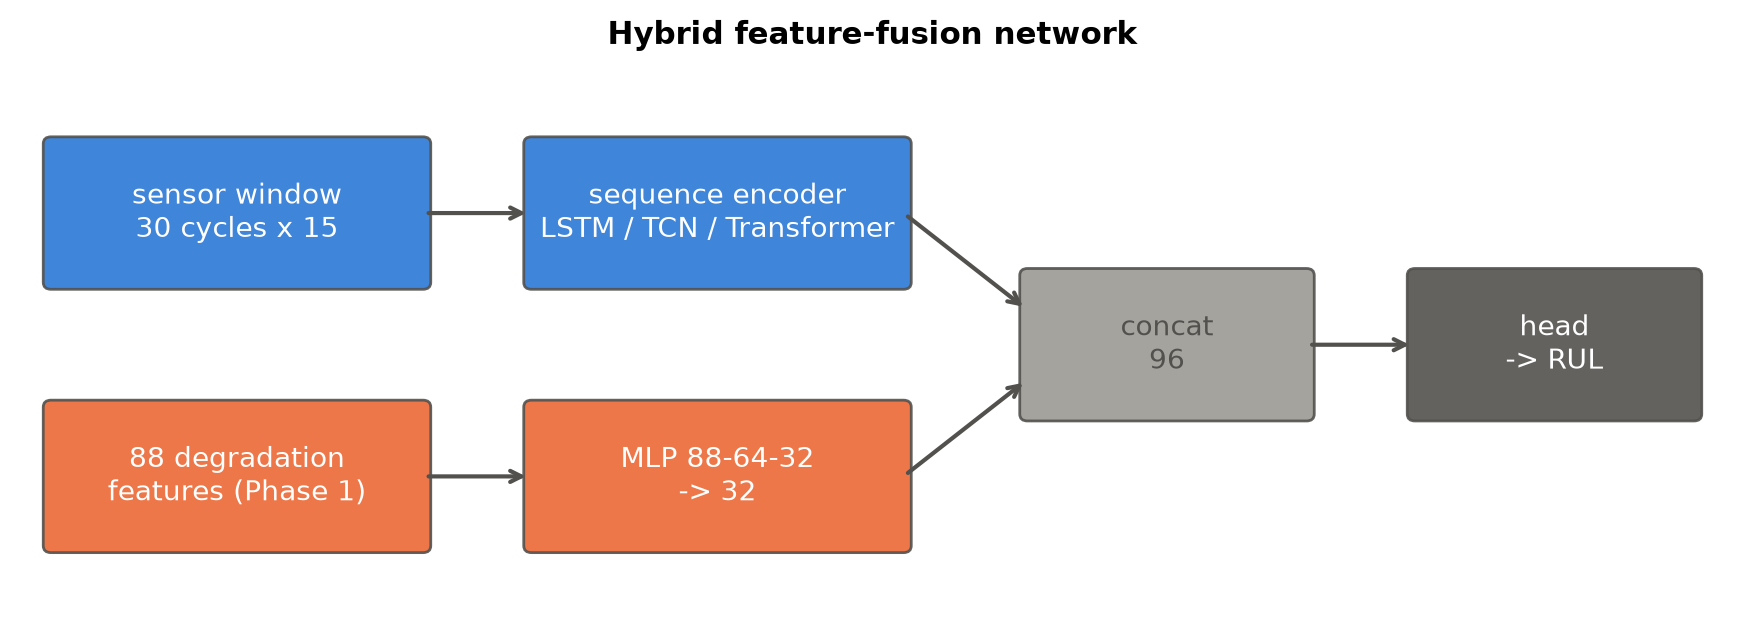
\includegraphics[width=\columnwidth]{08_hybrid_architecture.png}
  \caption{Hybrid feature-fusion network.}
  \label{fig:hybrid}
\end{figure}

\subsection{Results}
Table~\ref{tab:hybrid} reports the hybrid against its two branches, Phase~1's XGBoost, and the late-fusion average. With the LSTM encoder, the hybrid ($9.55\pm0.77$) is 4.5 cycles better than the best sequence model alone and 0.5 cycles better than the feature branch alone, so each branch contributes information. Joint training matters: averaging XGBoost and the Transformer scores 10.24, worse than XGBoost alone, while the hybrid beats the average with every encoder. Against XGBoost (9.26) the hybrid is close but not better: it wins on 2 of 5 folds, and averaged over three seeds (Section~\ref{sec:ablation}) its CV RMSE is about 9.7--10.0.

The gain is concentrated where it matters most. In the last 50 cycles before failure the hybrid's RMSE is 4.14 against 5.04 for XGBoost (18\% lower) and 7.20 for the Transformer alone. In the onset region it recovers almost all of the sequence model's weakness (14.31 vs.\ 19.07; XGBoost 13.80). Fast-degrading engines remain about 10 cycles late for both XGBoost and the hybrid, since both use the engine's age, which makes a fast degrader look too young to fail.

\begin{table}[t]
\centering
\small
\caption{Hybrid versus its parts (5-fold CV RMSE)}
\label{tab:hybrid}
\resizebox{\columnwidth}{!}{\begin{tabular}{lcc}
\toprule
Model & RMSE & RMSE, last 50 cycles \\
\midrule
Sequence alone (Transformer) & 13.05 & 7.20 \\
Feature branch alone (MLP) & 10.04 & -- \\
Average of XGBoost and Transformer & 10.24 & -- \\
XGBoost, engineered (Phase~1) & \textbf{9.26} & 5.04 \\
Hybrid, TCN encoder & 9.87 & -- \\
Hybrid, Transformer encoder & 9.74 & -- \\
Hybrid, LSTM encoder & 9.55 & \textbf{4.14} \\
\bottomrule
\end{tabular}}
\end{table}
